\documentclass[1p]{elsarticle_modified}
%\bibliographystyle{elsarticle-num}

%\usepackage[colorlinks]{hyperref}
%\usepackage{abbrmath_seonhwa} %\Abb, \Ascr, \Acal ,\Abf, \Afrak
\usepackage{amsfonts}
\usepackage{amssymb}
\usepackage{amsmath}
\usepackage{amsthm}
\usepackage{scalefnt}
\usepackage{amsbsy}
\usepackage{kotex}
\usepackage{caption}
\usepackage{subfig}
\usepackage{color}
\usepackage{graphicx}
\usepackage{xcolor} %% white, black, red, green, blue, cyan, magenta, yellow
\usepackage{float}
\usepackage{setspace}
\usepackage{hyperref}

\usepackage{tikz}
\usetikzlibrary{arrows}

\usepackage{multirow}
\usepackage{array} % fixed length table
\usepackage{hhline}

%%%%%%%%%%%%%%%%%%%%%
\makeatletter
\renewcommand*\env@matrix[1][\arraystretch]{%
	\edef\arraystretch{#1}%
	\hskip -\arraycolsep
	\let\@ifnextchar\new@ifnextchar
	\array{*\c@MaxMatrixCols c}}
\makeatother %https://tex.stackexchange.com/questions/14071/how-can-i-increase-the-line-spacing-in-a-matrix
%%%%%%%%%%%%%%%

\usepackage[normalem]{ulem}

\newcommand{\msout}[1]{\ifmmode\text{\sout{\ensuremath{#1}}}\else\sout{#1}\fi}
%SOURCE: \msout is \stkout macro in https://tex.stackexchange.com/questions/20609/strikeout-in-math-mode

\newcommand{\cancel}[1]{
	\ifmmode
	{\color{red}\msout{#1}}
	\else
	{\color{red}\sout{#1}}
	\fi
}

\newcommand{\add}[1]{
	{\color{blue}\uwave{#1}}
}

\newcommand{\replace}[2]{
	\ifmmode
	{\color{red}\msout{#1}}{\color{blue}\uwave{#2}}
	\else
	{\color{red}\sout{#1}}{\color{blue}\uwave{#2}}
	\fi
}

\newcommand{\Sol}{\mathcal{S}} %segment
\newcommand{\D}{D} %diagram
\newcommand{\A}{\mathcal{A}} %arc


%%%%%%%%%%%%%%%%%%%%%%%%%%%%%5 test

\def\sl{\operatorname{\textup{SL}}(2,\Cbb)}
\def\psl{\operatorname{\textup{PSL}}(2,\Cbb)}
\def\quan{\mkern 1mu \triangleright \mkern 1mu}

\theoremstyle{definition}
\newtheorem{thm}{Theorem}[section]
\newtheorem{prop}[thm]{Proposition}
\newtheorem{lem}[thm]{Lemma}
\newtheorem{ques}[thm]{Question}
\newtheorem{cor}[thm]{Corollary}
\newtheorem{defn}[thm]{Definition}
\newtheorem{exam}[thm]{Example}
\newtheorem{rmk}[thm]{Remark}
\newtheorem{alg}[thm]{Algorithm}

\newcommand{\I}{\sqrt{-1}}
\begin{document}

%\begin{frontmatter}
%
%\title{Boundary parabolic representations of knots up to 8 crossings}
%
%%% Group authors per affiliation:
%\author{Yunhi Cho} 
%\address{Department of Mathematics, University of Seoul, Seoul, Korea}
%\ead{yhcho@uos.ac.kr}
%
%
%\author{Seonhwa Kim} %\fnref{s_kim}}
%\address{Center for Geometry and Physics, Institute for Basic Science, Pohang, 37673, Korea}
%\ead{ryeona17@ibs.re.kr}
%
%\author{Hyuk Kim}
%\address{Department of Mathematical Sciences, Seoul National University, Seoul 08826, Korea}
%\ead{hyukkim@snu.ac.kr}
%
%\author{Seokbeom Yoon}
%\address{Department of Mathematical Sciences, Seoul National University, Seoul, 08826,  Korea}
%\ead{sbyoon15@snu.ac.kr}
%
%\begin{abstract}
%We find all boundary parabolic representation of knots up to 8 crossings.
%
%\end{abstract}
%\begin{keyword}
%    \MSC[2010] 57M25 
%\end{keyword}
%
%\end{frontmatter}

%\linenumbers
%\tableofcontents
%
\newcommand\colored[1]{\textcolor{white}{\rule[-0.35ex]{0.8em}{1.4ex}}\kern-0.8em\color{red} #1}%
%\newcommand\colored[1]{\textcolor{white}{ #1}\kern-2.17ex	\textcolor{white}{ #1}\kern-1.81ex	\textcolor{white}{ #1}\kern-2.15ex\color{red}#1	}

{\Large $\underline{12n_{0204}~(K12n_{0204})}$}

\setlength{\tabcolsep}{10pt}
\renewcommand{\arraystretch}{1.6}
\vspace{1cm}\begin{tabular}{m{100pt}>{\centering\arraybackslash}m{274pt}}
\multirow{5}{120pt}{
	\centering
	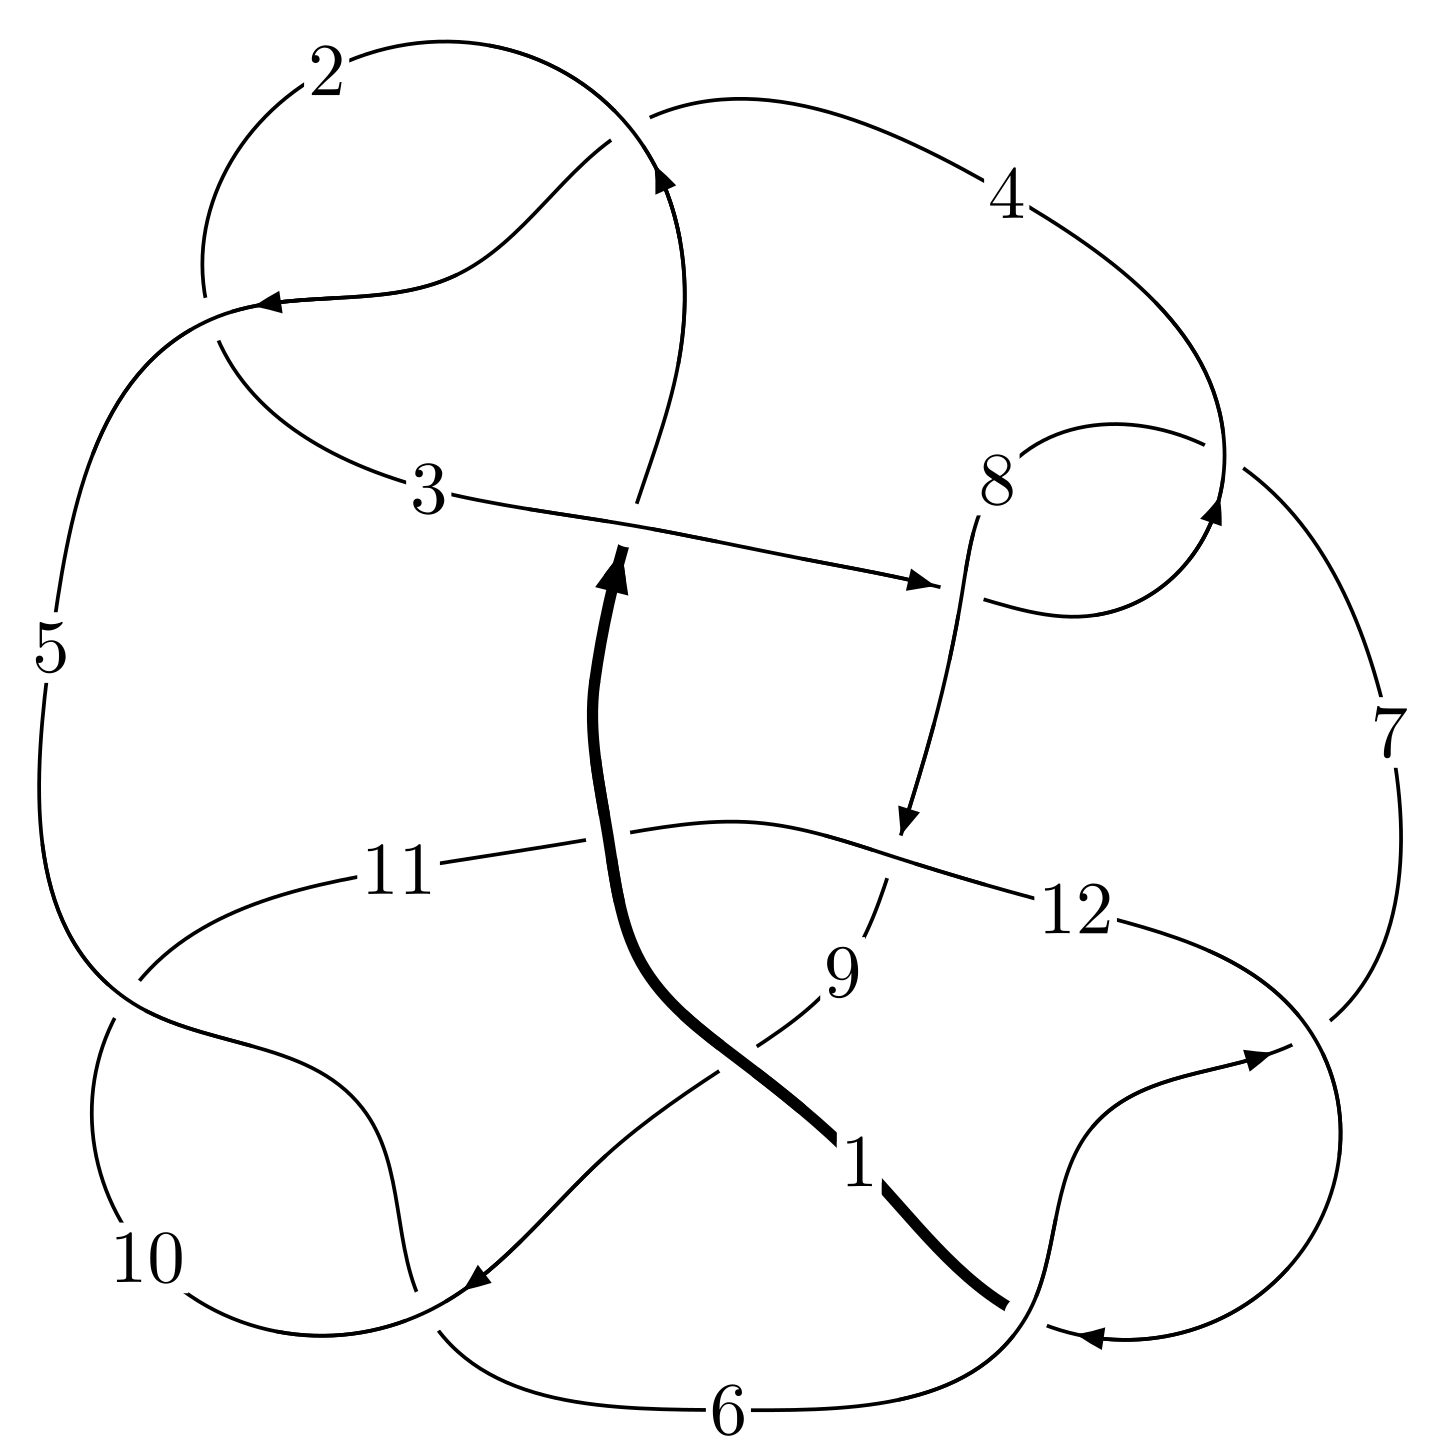
\includegraphics[width=112pt]{../../../GIT/diagram.site/Diagrams/png/2293_12n_0204.png}\\
\ \ \ A knot diagram\footnotemark}&
\allowdisplaybreaks
\textbf{Linearized knot diagam} \\
\cline{2-2}
 &
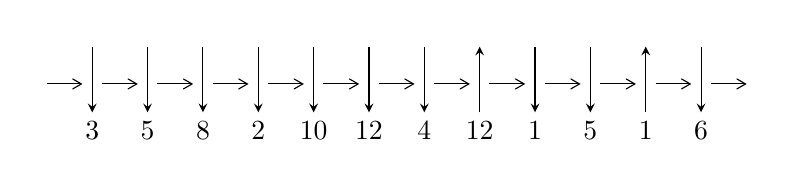
\begin{tikzpicture}[x=20pt, y=17pt]
	% nodes
	\node (C0) at (0, 0) {};
	\node (C1) at (1, 0) {};
	\node (C1U) at (1, +1) {};
	\node (C1D) at (1, -1) {3};

	\node (C2) at (2, 0) {};
	\node (C2U) at (2, +1) {};
	\node (C2D) at (2, -1) {5};

	\node (C3) at (3, 0) {};
	\node (C3U) at (3, +1) {};
	\node (C3D) at (3, -1) {8};

	\node (C4) at (4, 0) {};
	\node (C4U) at (4, +1) {};
	\node (C4D) at (4, -1) {2};

	\node (C5) at (5, 0) {};
	\node (C5U) at (5, +1) {};
	\node (C5D) at (5, -1) {10};

	\node (C6) at (6, 0) {};
	\node (C6U) at (6, +1) {};
	\node (C6D) at (6, -1) {12};

	\node (C7) at (7, 0) {};
	\node (C7U) at (7, +1) {};
	\node (C7D) at (7, -1) {4};

	\node (C8) at (8, 0) {};
	\node (C8U) at (8, +1) {};
	\node (C8D) at (8, -1) {12};

	\node (C9) at (9, 0) {};
	\node (C9U) at (9, +1) {};
	\node (C9D) at (9, -1) {1};

	\node (C10) at (10, 0) {};
	\node (C10U) at (10, +1) {};
	\node (C10D) at (10, -1) {5};

	\node (C11) at (11, 0) {};
	\node (C11U) at (11, +1) {};
	\node (C11D) at (11, -1) {1};

	\node (C12) at (12, 0) {};
	\node (C12U) at (12, +1) {};
	\node (C12D) at (12, -1) {6};
	\node (C13) at (13, 0) {};

	% arrows
	\draw[->,>={angle 60}]
	(C0) edge (C1) (C1) edge (C2) (C2) edge (C3) (C3) edge (C4) (C4) edge (C5) (C5) edge (C6) (C6) edge (C7) (C7) edge (C8) (C8) edge (C9) (C9) edge (C10) (C10) edge (C11) (C11) edge (C12) (C12) edge (C13) ;	\draw[->,>=stealth]
	(C1U) edge (C1D) (C2U) edge (C2D) (C3U) edge (C3D) (C4U) edge (C4D) (C5U) edge (C5D) (C6U) edge (C6D) (C7U) edge (C7D) (C8D) edge (C8U) (C9U) edge (C9D) (C10U) edge (C10D) (C11D) edge (C11U) (C12U) edge (C12D) ;
	\end{tikzpicture} \\
\hhline{~~} \\& 
\textbf{Solving Sequence} \\ \cline{2-2} 
 &
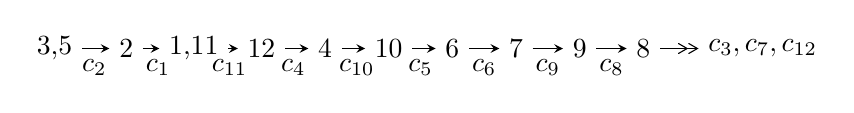
\begin{tikzpicture}[x=23pt, y=7pt]
	% node
	\node (A0) at (-1/8, 0) {3,5};
	\node (A1) at (1, 0) {2};
	\node (A2) at (33/16, 0) {1,11};
	\node (A3) at (25/8, 0) {12};
	\node (A4) at (33/8, 0) {4};
	\node (A5) at (41/8, 0) {10};
	\node (A6) at (49/8, 0) {6};
	\node (A7) at (57/8, 0) {7};
	\node (A8) at (65/8, 0) {9};
	\node (A9) at (73/8, 0) {8};
	\node (C1) at (1/2, -1) {$c_{2}$};
	\node (C2) at (3/2, -1) {$c_{1}$};
	\node (C3) at (21/8, -1) {$c_{11}$};
	\node (C4) at (29/8, -1) {$c_{4}$};
	\node (C5) at (37/8, -1) {$c_{10}$};
	\node (C6) at (45/8, -1) {$c_{5}$};
	\node (C7) at (53/8, -1) {$c_{6}$};
	\node (C8) at (61/8, -1) {$c_{9}$};
	\node (C9) at (69/8, -1) {$c_{8}$};
	\node (A10) at (11, 0) {$c_{3},c_{7},c_{12}$};

	% edge
	\draw[->,>=stealth]	
	(A0) edge (A1) (A1) edge (A2) (A2) edge (A3) (A3) edge (A4) (A4) edge (A5) (A5) edge (A6) (A6) edge (A7) (A7) edge (A8) (A8) edge (A9) ;
	\draw[->>,>={angle 60}]	
	(A9) edge (A10);
\end{tikzpicture} \\ 

\end{tabular} \\

\footnotetext{
The image of knot diagram is generated by the software ``\textbf{Draw programme}" developed by Andrew Bartholomew(\url{http://www.layer8.co.uk/maths/draw/index.htm\#Running-draw}), where we modified some parts for our purpose(\url{https://github.com/CATsTAILs/LinksPainter}).
}\phantom \\ \newline 
\centering \textbf{Ideals for irreducible components\footnotemark of $X_{\text{par}}$} 
 
\begin{align*}
I^u_{1}&=\langle 
-409562441 u^{28}-633138331 u^{27}+\cdots+1278981878 b+1495358594,\\
\phantom{I^u_{1}}&\phantom{= \langle  }-649542429 u^{28}-1056906370 u^{27}+\cdots+2557963756 a-48242973,\;u^{29}+2 u^{28}+\cdots+5 u-4\rangle \\
I^u_{2}&=\langle 
u^{14} a- u^{14}+\cdots+b-1,\;-2 u^{14}- u^{13}+\cdots- a+3,\\
\phantom{I^u_{2}}&\phantom{= \langle  }u^{15}+u^{14}-4 u^{13}-5 u^{12}+6 u^{11}+10 u^{10}-7 u^8-8 u^7-4 u^6+6 u^5+8 u^4+2 u^3-2 u^2-2 u-1\rangle \\
I^u_{3}&=\langle 
u^4 a+u^3 a- u^4- u^3- a u+b- a+u,\;u^5-2 u^3+a^2- u^2+2 u+1,\;u^6+u^5- u^4-2 u^3+u+1\rangle \\
I^u_{4}&=\langle 
2 b+3,\;a+1,\;u-1\rangle \\
\\
\end{align*}
\raggedright * 4 irreducible components of $\dim_{\mathbb{C}}=0$, with total 72 representations.\\
\footnotetext{All coefficients of polynomials are rational numbers. But the coefficients are sometimes approximated in decimal forms when there is not enough margin.}
\newpage
\renewcommand{\arraystretch}{1}
\centering \section*{I. $I^u_{1}= \langle -4.10\times10^{8} u^{28}-6.33\times10^{8} u^{27}+\cdots+1.28\times10^{9} b+1.50\times10^{9},\;-6.50\times10^{8} u^{28}-1.06\times10^{9} u^{27}+\cdots+2.56\times10^{9} a-4.82\times10^{7},\;u^{29}+2 u^{28}+\cdots+5 u-4 \rangle$}
\flushleft \textbf{(i) Arc colorings}\\
\begin{tabular}{m{7pt} m{180pt} m{7pt} m{180pt} }
\flushright $a_{3}=$&$\begin{pmatrix}1\\0\end{pmatrix}$ \\
\flushright $a_{5}=$&$\begin{pmatrix}0\\u\end{pmatrix}$ \\
\flushright $a_{2}=$&$\begin{pmatrix}1\\- u^2\end{pmatrix}$ \\
\flushright $a_{1}=$&$\begin{pmatrix}- u^2+1\\- u^2\end{pmatrix}$ \\
\flushright $a_{11}=$&$\begin{pmatrix}0.253929 u^{28}+0.413183 u^{27}+\cdots+3.78605 u+0.0188599\\0.320225 u^{28}+0.495033 u^{27}+\cdots+1.86204 u-1.16918\end{pmatrix}$ \\
\flushright $a_{12}=$&$\begin{pmatrix}0.253151 u^{28}+0.268291 u^{27}+\cdots+2.54838 u+0.206314\\0.0347611 u^{28}+0.0691866 u^{27}+\cdots-0.718788 u-0.0155112\end{pmatrix}$ \\
\flushright $a_{4}=$&$\begin{pmatrix}u\\- u^3+u\end{pmatrix}$ \\
\flushright $a_{10}=$&$\begin{pmatrix}0.253929 u^{28}+0.413183 u^{27}+\cdots+3.78605 u+0.0188599\\0.265953 u^{28}+0.469651 u^{27}+\cdots+0.372941 u-0.790474\end{pmatrix}$ \\
\flushright $a_{6}=$&$\begin{pmatrix}-0.241553 u^{28}-0.198421 u^{27}+\cdots-2.06949 u+0.135383\\0.0507414 u^{28}+0.0659434 u^{27}+\cdots+1.51952 u-0.265184\end{pmatrix}$ \\
\flushright $a_{7}=$&$\begin{pmatrix}-0.482352 u^{28}-0.389873 u^{27}+\cdots-4.05885 u+0.333349\\0.0518322 u^{28}+0.0860020 u^{27}+\cdots+1.78896 u-0.341645\end{pmatrix}$ \\
\flushright $a_{9}=$&$\begin{pmatrix}0.246071 u^{28}+0.0868173 u^{27}+\cdots+1.21395 u+0.481140\\-0.0746592 u^{28}-0.176612 u^{27}+\cdots-2.68612 u+0.591964\end{pmatrix}$ \\
\flushright $a_{8}=$&$\begin{pmatrix}0.487395 u^{28}+0.426835 u^{27}+\cdots+3.80650 u-0.325257\\-0.00202308 u^{28}-0.00908992 u^{27}+\cdots-1.92712 u+0.242240\end{pmatrix}$\\&\end{tabular}
\flushleft \textbf{(ii) Obstruction class $= -1$}\\~\\
\flushleft \textbf{(iii) Cusp Shapes $= \frac{1071754917}{2557963756} u^{28}-\frac{75682913}{2557963756} u^{27}+\cdots+\frac{8446888807}{2557963756} u-\frac{9796598069}{639490939}$}\\~\\
\newpage\renewcommand{\arraystretch}{1}
\flushleft \textbf{(iv) u-Polynomials at the component}\newline \\
\begin{tabular}{m{50pt}|m{274pt}}
Crossings & \hspace{64pt}u-Polynomials at each crossing \\
\hline $$\begin{aligned}c_{1}\end{aligned}$$&$\begin{aligned}
&u^{29}+16 u^{28}+\cdots+209 u+16
\end{aligned}$\\
\hline $$\begin{aligned}c_{2},c_{4}\end{aligned}$$&$\begin{aligned}
&u^{29}-2 u^{28}+\cdots+5 u+4
\end{aligned}$\\
\hline $$\begin{aligned}c_{3},c_{7}\end{aligned}$$&$\begin{aligned}
&u^{29}+3 u^{28}+\cdots+18 u+8
\end{aligned}$\\
\hline $$\begin{aligned}c_{5},c_{6},c_{10}\\c_{12}\end{aligned}$$&$\begin{aligned}
&u^{29}+u^{28}+\cdots+2 u+1
\end{aligned}$\\
\hline $$\begin{aligned}c_{8},c_{11}\end{aligned}$$&$\begin{aligned}
&u^{29}-5 u^{28}+\cdots-6 u+1
\end{aligned}$\\
\hline $$\begin{aligned}c_{9}\end{aligned}$$&$\begin{aligned}
&u^{29}+26 u^{28}+\cdots+376832 u+32768
\end{aligned}$\\
\hline
\end{tabular}\\~\\
\newpage\renewcommand{\arraystretch}{1}
\flushleft \textbf{(v) Riley Polynomials at the component}\newline \\
\begin{tabular}{m{50pt}|m{274pt}}
Crossings & \hspace{64pt}Riley Polynomials at each crossing \\
\hline $$\begin{aligned}c_{1}\end{aligned}$$&$\begin{aligned}
&y^{29}-4 y^{28}+\cdots+21313 y-256
\end{aligned}$\\
\hline $$\begin{aligned}c_{2},c_{4}\end{aligned}$$&$\begin{aligned}
&y^{29}-16 y^{28}+\cdots+209 y-16
\end{aligned}$\\
\hline $$\begin{aligned}c_{3},c_{7}\end{aligned}$$&$\begin{aligned}
&y^{29}+9 y^{28}+\cdots-140 y-64
\end{aligned}$\\
\hline $$\begin{aligned}c_{5},c_{6},c_{10}\\c_{12}\end{aligned}$$&$\begin{aligned}
&y^{29}+5 y^{28}+\cdots-6 y-1
\end{aligned}$\\
\hline $$\begin{aligned}c_{8},c_{11}\end{aligned}$$&$\begin{aligned}
&y^{29}+45 y^{28}+\cdots+6 y-1
\end{aligned}$\\
\hline $$\begin{aligned}c_{9}\end{aligned}$$&$\begin{aligned}
&y^{29}-16 y^{28}+\cdots+6174015488 y-1073741824
\end{aligned}$\\
\hline
\end{tabular}\\~\\
\newpage\flushleft \textbf{(vi) Complex Volumes and Cusp Shapes}
$$\begin{array}{c|c|c}  
\text{Solutions to }I^u_{1}& \I (\text{vol} + \sqrt{-1}CS) & \text{Cusp shape}\\
 \hline 
\begin{aligned}
u &= -0.960613 + 0.170294 I \\
a &= -1.129440 - 0.468149 I \\
b &= -1.63701 - 0.14149 I\end{aligned}
 & -3.34627 + 0.60911 I & -7.67402 - 10.34191 I \\ \hline\begin{aligned}
u &= -0.960613 - 0.170294 I \\
a &= -1.129440 + 0.468149 I \\
b &= -1.63701 + 0.14149 I\end{aligned}
 & -3.34627 - 0.60911 I & -7.67402 + 10.34191 I \\ \hline\begin{aligned}
u &= \phantom{-}0.829481 + 0.498753 I \\
a &= \phantom{-}0.851038 + 0.266459 I \\
b &= \phantom{-}1.25630 - 0.93003 I\end{aligned}
 & -0.95125 - 3.42018 I & -9.12436 + 7.13905 I \\ \hline\begin{aligned}
u &= \phantom{-}0.829481 - 0.498753 I \\
a &= \phantom{-}0.851038 - 0.266459 I \\
b &= \phantom{-}1.25630 + 0.93003 I\end{aligned}
 & -0.95125 + 3.42018 I & -9.12436 - 7.13905 I \\ \hline\begin{aligned}
u &= -0.555934 + 0.787790 I \\
a &= -0.385011 + 0.878403 I \\
b &= -0.547815 - 0.259593 I\end{aligned}
 & \phantom{-}3.91212 - 3.07296 I & -3.58580 + 5.16956 I \\ \hline\begin{aligned}
u &= -0.555934 - 0.787790 I \\
a &= -0.385011 - 0.878403 I \\
b &= -0.547815 + 0.259593 I\end{aligned}
 & \phantom{-}3.91212 + 3.07296 I & -3.58580 - 5.16956 I \\ \hline\begin{aligned}
u &= -0.133622 + 0.942757 I \\
a &= -1.05744 + 1.03712 I \\
b &= -0.400359 - 0.621002 I\end{aligned}
 & -3.40148 - 10.10230 I & -5.65840 + 6.34779 I \\ \hline\begin{aligned}
u &= -0.133622 - 0.942757 I \\
a &= -1.05744 - 1.03712 I \\
b &= -0.400359 + 0.621002 I\end{aligned}
 & -3.40148 + 10.10230 I & -5.65840 - 6.34779 I \\ \hline\begin{aligned}
u &= -0.482129 + 0.757528 I \\
a &= \phantom{-}0.760914 - 0.157398 I \\
b &= \phantom{-}0.683226 + 0.243077 I\end{aligned}
 & \phantom{-}3.66760 - 0.05333 I & -4.59541 - 3.69602 I \\ \hline\begin{aligned}
u &= -0.482129 - 0.757528 I \\
a &= \phantom{-}0.760914 + 0.157398 I \\
b &= \phantom{-}0.683226 - 0.243077 I\end{aligned}
 & \phantom{-}3.66760 + 0.05333 I & -4.59541 + 3.69602 I\\
 \hline 
 \end{array}$$\newpage$$\begin{array}{c|c|c}  
\text{Solutions to }I^u_{1}& \I (\text{vol} + \sqrt{-1}CS) & \text{Cusp shape}\\
 \hline 
\begin{aligned}
u &= \phantom{-}0.819144 + 0.362327 I \\
a &= \phantom{-}0.087730 - 0.590172 I \\
b &= -0.776429 + 0.138255 I\end{aligned}
 & -0.751059 - 0.353134 I & -9.39424 - 1.40493 I \\ \hline\begin{aligned}
u &= \phantom{-}0.819144 - 0.362327 I \\
a &= \phantom{-}0.087730 + 0.590172 I \\
b &= -0.776429 - 0.138255 I\end{aligned}
 & -0.751059 + 0.353134 I & -9.39424 + 1.40493 I \\ \hline\begin{aligned}
u &= \phantom{-}0.121290 + 0.842756 I \\
a &= -1.00456 - 1.22447 I \\
b &= -0.539181 + 0.622092 I\end{aligned}
 & -4.45862 + 3.60692 I & -7.22386 - 2.01130 I \\ \hline\begin{aligned}
u &= \phantom{-}0.121290 - 0.842756 I \\
a &= -1.00456 + 1.22447 I \\
b &= -0.539181 - 0.622092 I\end{aligned}
 & -4.45862 - 3.60692 I & -7.22386 + 2.01130 I \\ \hline\begin{aligned}
u &= -1.002290 + 0.666485 I \\
a &= \phantom{-}0.794138 - 0.363712 I \\
b &= \phantom{-}1.64106 + 0.14073 I\end{aligned}
 & \phantom{-}2.60025 + 8.50017 I & -5.17138 - 9.83055 I \\ \hline\begin{aligned}
u &= -1.002290 - 0.666485 I \\
a &= \phantom{-}0.794138 + 0.363712 I \\
b &= \phantom{-}1.64106 - 0.14073 I\end{aligned}
 & \phantom{-}2.60025 - 8.50017 I & -5.17138 + 9.83055 I \\ \hline\begin{aligned}
u &= -1.064380 + 0.598303 I \\
a &= -0.159509 + 0.533064 I \\
b &= -0.638339 - 0.004258 I\end{aligned}
 & \phantom{-}1.93242 + 5.18468 I & -8.47176 - 2.14374 I \\ \hline\begin{aligned}
u &= -1.064380 - 0.598303 I \\
a &= -0.159509 - 0.533064 I \\
b &= -0.638339 + 0.004258 I\end{aligned}
 & \phantom{-}1.93242 - 5.18468 I & -8.47176 + 2.14374 I \\ \hline\begin{aligned}
u &= \phantom{-}1.230540 + 0.053330 I \\
a &= -0.440769 + 0.411058 I \\
b &= -1.154760 + 0.333664 I\end{aligned}
 & -2.23909 + 1.32557 I & -7.93584 - 5.22491 I \\ \hline\begin{aligned}
u &= \phantom{-}1.230540 - 0.053330 I \\
a &= -0.440769 - 0.411058 I \\
b &= -1.154760 - 0.333664 I\end{aligned}
 & -2.23909 - 1.32557 I & -7.93584 + 5.22491 I\\
 \hline 
 \end{array}$$\newpage$$\begin{array}{c|c|c}  
\text{Solutions to }I^u_{1}& \I (\text{vol} + \sqrt{-1}CS) & \text{Cusp shape}\\
 \hline 
\begin{aligned}
u &= -1.243450 + 0.397204 I \\
a &= -0.541600 - 0.973717 I \\
b &= -1.67988 - 0.94005 I\end{aligned}
 & -8.59540 + 0.64697 I & -11.02522 - 1.67463 I \\ \hline\begin{aligned}
u &= -1.243450 - 0.397204 I \\
a &= -0.541600 + 0.973717 I \\
b &= -1.67988 + 0.94005 I\end{aligned}
 & -8.59540 - 0.64697 I & -11.02522 + 1.67463 I \\ \hline\begin{aligned}
u &= \phantom{-}1.215230 + 0.518861 I \\
a &= \phantom{-}0.943218 + 0.506066 I \\
b &= \phantom{-}2.90492 + 0.42900 I\end{aligned}
 & -7.70776 - 8.57292 I & -9.65881 + 5.33629 I \\ \hline\begin{aligned}
u &= \phantom{-}1.215230 - 0.518861 I \\
a &= \phantom{-}0.943218 - 0.506066 I \\
b &= \phantom{-}2.90492 - 0.42900 I\end{aligned}
 & -7.70776 + 8.57292 I & -9.65881 - 5.33629 I \\ \hline\begin{aligned}
u &= -1.252950 + 0.545209 I \\
a &= \phantom{-}0.925713 - 0.557598 I \\
b &= \phantom{-}2.79765 - 0.77731 I\end{aligned}
 & -6.8135 + 15.4607 I & -8.47000 - 9.06787 I \\ \hline\begin{aligned}
u &= -1.252950 - 0.545209 I \\
a &= \phantom{-}0.925713 + 0.557598 I \\
b &= \phantom{-}2.79765 + 0.77731 I\end{aligned}
 & -6.8135 - 15.4607 I & -8.47000 + 9.06787 I \\ \hline\begin{aligned}
u &= \phantom{-}1.313260 + 0.385635 I \\
a &= -0.416958 + 0.934515 I \\
b &= -1.47424 + 1.05397 I\end{aligned}
 & -8.00289 + 5.49028 I & -9.85377 - 4.12172 I \\ \hline\begin{aligned}
u &= \phantom{-}1.313260 - 0.385635 I \\
a &= -0.416958 - 0.934515 I \\
b &= -1.47424 - 1.05397 I\end{aligned}
 & -8.00289 - 5.49028 I & -9.85377 + 4.12172 I \\ \hline\begin{aligned}
u &= \phantom{-}0.332840\phantom{ +0.000000I} \\
a &= \phantom{-}1.29507\phantom{ +0.000000I} \\
b &= -0.370297\phantom{ +0.000000I}\end{aligned}
 & -0.777392\phantom{ +0.000000I} & -12.5640\phantom{ +0.000000I}\\
 \hline 
 \end{array}$$\newpage\newpage\renewcommand{\arraystretch}{1}
\centering \section*{II. $I^u_{2}= \langle u^{14} a- u^{14}+\cdots+b-1,\;-2 u^{14}- u^{13}+\cdots- a+3,\;u^{15}+u^{14}+\cdots-2 u-1 \rangle$}
\flushleft \textbf{(i) Arc colorings}\\
\begin{tabular}{m{7pt} m{180pt} m{7pt} m{180pt} }
\flushright $a_{3}=$&$\begin{pmatrix}1\\0\end{pmatrix}$ \\
\flushright $a_{5}=$&$\begin{pmatrix}0\\u\end{pmatrix}$ \\
\flushright $a_{2}=$&$\begin{pmatrix}1\\- u^2\end{pmatrix}$ \\
\flushright $a_{1}=$&$\begin{pmatrix}- u^2+1\\- u^2\end{pmatrix}$ \\
\flushright $a_{11}=$&$\begin{pmatrix}a\\- u^{14} a+u^{14}+\cdots+u+1\end{pmatrix}$ \\
\flushright $a_{12}=$&$\begin{pmatrix}u^6 a-2 u^4 a+u^2 a- u^2+a+1\\- u^{14} a+u^{14}+\cdots+u+1\end{pmatrix}$ \\
\flushright $a_{4}=$&$\begin{pmatrix}u\\- u^3+u\end{pmatrix}$ \\
\flushright $a_{10}=$&$\begin{pmatrix}a\\- u^{14} a+u^{14}+\cdots+u+1\end{pmatrix}$ \\
\flushright $a_{6}=$&$\begin{pmatrix}u^{14}+u^{13}+\cdots- u-2\\- u^{13} a- u^{13}+\cdots- a-1\end{pmatrix}$ \\
\flushright $a_{7}=$&$\begin{pmatrix}- u^{11}+4 u^9-6 u^7+2 u^5+3 u^3-2 u\\- u^{11}+3 u^9-4 u^7+u^5+u^3- u\end{pmatrix}$ \\
\flushright $a_{9}=$&$\begin{pmatrix}- u^2+a+1\\- u^{14} a+u^{14}+\cdots+u+1\end{pmatrix}$ \\
\flushright $a_{8}=$&$\begin{pmatrix}u^{14}-5 u^{12}+10 u^{10}-7 u^8-4 u^6+8 u^4-2 u^2-1\\u^{14}-4 u^{12}+7 u^{10}-4 u^8-2 u^6+4 u^4- u^2\end{pmatrix}$\\&\end{tabular}
\flushleft \textbf{(ii) Obstruction class $= -1$}\\~\\
\flushleft \textbf{(iii) Cusp Shapes $= -4 u^{13}+16 u^{11}+4 u^{10}-28 u^9-12 u^8+12 u^7+16 u^6+16 u^5-24 u^3-8 u^2-2$}\\~\\
\newpage\renewcommand{\arraystretch}{1}
\flushleft \textbf{(iv) u-Polynomials at the component}\newline \\
\begin{tabular}{m{50pt}|m{274pt}}
Crossings & \hspace{64pt}u-Polynomials at each crossing \\
\hline $$\begin{aligned}c_{1}\end{aligned}$$&$\begin{aligned}
&(u^{15}+9 u^{14}+\cdots-4 u^2+1)^{2}
\end{aligned}$\\
\hline $$\begin{aligned}c_{2},c_{4}\end{aligned}$$&$\begin{aligned}
&(u^{15}- u^{14}+\cdots-2 u+1)^{2}
\end{aligned}$\\
\hline $$\begin{aligned}c_{3},c_{7}\end{aligned}$$&$\begin{aligned}
&(u^{15}- u^{14}+\cdots+2 u-1)^{2}
\end{aligned}$\\
\hline $$\begin{aligned}c_{5},c_{6},c_{10}\\c_{12}\end{aligned}$$&$\begin{aligned}
&u^{30}-3 u^{29}+\cdots-30 u+9
\end{aligned}$\\
\hline $$\begin{aligned}c_{8},c_{11}\end{aligned}$$&$\begin{aligned}
&u^{30}-11 u^{29}+\cdots-1296 u+81
\end{aligned}$\\
\hline $$\begin{aligned}c_{9}\end{aligned}$$&$\begin{aligned}
&(u-1)^{30}
\end{aligned}$\\
\hline
\end{tabular}\\~\\
\newpage\renewcommand{\arraystretch}{1}
\flushleft \textbf{(v) Riley Polynomials at the component}\newline \\
\begin{tabular}{m{50pt}|m{274pt}}
Crossings & \hspace{64pt}Riley Polynomials at each crossing \\
\hline $$\begin{aligned}c_{1}\end{aligned}$$&$\begin{aligned}
&(y^{15}-5 y^{14}+\cdots+8 y-1)^{2}
\end{aligned}$\\
\hline $$\begin{aligned}c_{2},c_{4}\end{aligned}$$&$\begin{aligned}
&(y^{15}-9 y^{14}+\cdots+4 y^2-1)^{2}
\end{aligned}$\\
\hline $$\begin{aligned}c_{3},c_{7}\end{aligned}$$&$\begin{aligned}
&(y^{15}+3 y^{14}+\cdots+8 y^2-1)^{2}
\end{aligned}$\\
\hline $$\begin{aligned}c_{5},c_{6},c_{10}\\c_{12}\end{aligned}$$&$\begin{aligned}
&y^{30}+11 y^{29}+\cdots+1296 y+81
\end{aligned}$\\
\hline $$\begin{aligned}c_{8},c_{11}\end{aligned}$$&$\begin{aligned}
&y^{30}+15 y^{29}+\cdots-73224 y+6561
\end{aligned}$\\
\hline $$\begin{aligned}c_{9}\end{aligned}$$&$\begin{aligned}
&(y-1)^{30}
\end{aligned}$\\
\hline
\end{tabular}\\~\\
\newpage\flushleft \textbf{(vi) Complex Volumes and Cusp Shapes}
$$\begin{array}{c|c|c}  
\text{Solutions to }I^u_{2}& \I (\text{vol} + \sqrt{-1}CS) & \text{Cusp shape}\\
 \hline 
\begin{aligned}
u &= -0.023100 + 0.900040 I \\
a &= \phantom{-}0.825316 + 1.129310 I \\
b &= \phantom{-}0.286301 - 0.445204 I\end{aligned}
 & -4.73497 - 3.25615 I & -7.67133 + 2.40088 I \\ \hline\begin{aligned}
u &= -0.023100 + 0.900040 I \\
a &= \phantom{-}0.98422 - 1.08773 I \\
b &= \phantom{-}0.164746 + 0.352495 I\end{aligned}
 & -4.73497 - 3.25615 I & -7.67133 + 2.40088 I \\ \hline\begin{aligned}
u &= -0.023100 - 0.900040 I \\
a &= \phantom{-}0.825316 - 1.129310 I \\
b &= \phantom{-}0.286301 + 0.445204 I\end{aligned}
 & -4.73497 + 3.25615 I & -7.67133 - 2.40088 I \\ \hline\begin{aligned}
u &= -0.023100 - 0.900040 I \\
a &= \phantom{-}0.98422 + 1.08773 I \\
b &= \phantom{-}0.164746 - 0.352495 I\end{aligned}
 & -4.73497 + 3.25615 I & -7.67133 - 2.40088 I \\ \hline\begin{aligned}
u &= \phantom{-}0.863978\phantom{ +0.000000I} \\
a &= \phantom{-}0.126771 + 1.178080 I \\
b &= \phantom{-}3.66551 - 2.58901 I\end{aligned}
 & \phantom{-}2.03422\phantom{ +0.000000I} & -12.4840\phantom{ +0.000000I} \\ \hline\begin{aligned}
u &= \phantom{-}0.863978\phantom{ +0.000000I} \\
a &= \phantom{-}0.126771 - 1.178080 I \\
b &= \phantom{-}3.66551 + 2.58901 I\end{aligned}
 & \phantom{-}2.03422\phantom{ +0.000000I} & -12.4840\phantom{ +0.000000I} \\ \hline\begin{aligned}
u &= \phantom{-}1.093890 + 0.311098 I \\
a &= -0.297631 - 0.955829 I \\
b &= -1.62293 - 0.54486 I\end{aligned}
 & -0.109911 - 1.108490 I & -11.51398 + 0.68443 I \\ \hline\begin{aligned}
u &= \phantom{-}1.093890 + 0.311098 I \\
a &= \phantom{-}0.197813 + 0.275213 I \\
b &= \phantom{-}0.45469 + 1.92439 I\end{aligned}
 & -0.109911 - 1.108490 I & -11.51398 + 0.68443 I \\ \hline\begin{aligned}
u &= \phantom{-}1.093890 - 0.311098 I \\
a &= -0.297631 + 0.955829 I \\
b &= -1.62293 + 0.54486 I\end{aligned}
 & -0.109911 + 1.108490 I & -11.51398 - 0.68443 I \\ \hline\begin{aligned}
u &= \phantom{-}1.093890 - 0.311098 I \\
a &= \phantom{-}0.197813 - 0.275213 I \\
b &= \phantom{-}0.45469 - 1.92439 I\end{aligned}
 & -0.109911 + 1.108490 I & -11.51398 - 0.68443 I\\
 \hline 
 \end{array}$$\newpage$$\begin{array}{c|c|c}  
\text{Solutions to }I^u_{2}& \I (\text{vol} + \sqrt{-1}CS) & \text{Cusp shape}\\
 \hline 
\begin{aligned}
u &= -0.747479 + 0.391613 I \\
a &= \phantom{-}1.023110 - 0.862412 I \\
b &= \phantom{-}1.63828 - 1.05509 I\end{aligned}
 & \phantom{-}4.53214 + 1.75942 I & -1.14915 - 5.01461 I \\ \hline\begin{aligned}
u &= -0.747479 + 0.391613 I \\
a &= -0.42847 + 1.44786 I \\
b &= \phantom{-}0.248041 - 0.151767 I\end{aligned}
 & \phantom{-}4.53214 + 1.75942 I & -1.14915 - 5.01461 I \\ \hline\begin{aligned}
u &= -0.747479 - 0.391613 I \\
a &= \phantom{-}1.023110 + 0.862412 I \\
b &= \phantom{-}1.63828 + 1.05509 I\end{aligned}
 & \phantom{-}4.53214 - 1.75942 I & -1.14915 + 5.01461 I \\ \hline\begin{aligned}
u &= -0.747479 - 0.391613 I \\
a &= -0.42847 - 1.44786 I \\
b &= \phantom{-}0.248041 + 0.151767 I\end{aligned}
 & \phantom{-}4.53214 - 1.75942 I & -1.14915 + 5.01461 I \\ \hline\begin{aligned}
u &= -1.070290 + 0.443484 I \\
a &= -0.592827 + 0.959612 I \\
b &= -1.162130 + 0.705596 I\end{aligned}
 & \phantom{-}0.87635 + 5.68434 I & -8.20490 - 7.47679 I \\ \hline\begin{aligned}
u &= -1.070290 + 0.443484 I \\
a &= \phantom{-}0.643980 - 0.010296 I \\
b &= \phantom{-}1.27621 - 1.00477 I\end{aligned}
 & \phantom{-}0.87635 + 5.68434 I & -8.20490 - 7.47679 I \\ \hline\begin{aligned}
u &= -1.070290 - 0.443484 I \\
a &= -0.592827 - 0.959612 I \\
b &= -1.162130 - 0.705596 I\end{aligned}
 & \phantom{-}0.87635 - 5.68434 I & -8.20490 + 7.47679 I \\ \hline\begin{aligned}
u &= -1.070290 - 0.443484 I \\
a &= \phantom{-}0.643980 + 0.010296 I \\
b &= \phantom{-}1.27621 + 1.00477 I\end{aligned}
 & \phantom{-}0.87635 - 5.68434 I & -8.20490 + 7.47679 I \\ \hline\begin{aligned}
u &= \phantom{-}1.268720 + 0.457284 I \\
a &= -0.923717 - 0.340768 I \\
b &= -2.59581 - 0.49906 I\end{aligned}
 & -8.68612 - 1.54935 I & -11.09602 + 0.66420 I \\ \hline\begin{aligned}
u &= \phantom{-}1.268720 + 0.457284 I \\
a &= \phantom{-}0.523167 - 0.819566 I \\
b &= \phantom{-}1.44899 - 1.21103 I\end{aligned}
 & -8.68612 - 1.54935 I & -11.09602 + 0.66420 I\\
 \hline 
 \end{array}$$\newpage$$\begin{array}{c|c|c}  
\text{Solutions to }I^u_{2}& \I (\text{vol} + \sqrt{-1}CS) & \text{Cusp shape}\\
 \hline 
\begin{aligned}
u &= \phantom{-}1.268720 - 0.457284 I \\
a &= -0.923717 + 0.340768 I \\
b &= -2.59581 + 0.49906 I\end{aligned}
 & -8.68612 + 1.54935 I & -11.09602 - 0.66420 I \\ \hline\begin{aligned}
u &= \phantom{-}1.268720 - 0.457284 I \\
a &= \phantom{-}0.523167 + 0.819566 I \\
b &= \phantom{-}1.44899 + 1.21103 I\end{aligned}
 & -8.68612 + 1.54935 I & -11.09602 - 0.66420 I \\ \hline\begin{aligned}
u &= -1.260410 + 0.482704 I \\
a &= \phantom{-}0.621138 + 0.785123 I \\
b &= \phantom{-}1.74021 + 0.98052 I\end{aligned}
 & -8.49724 + 8.19235 I & -10.69502 - 5.35870 I \\ \hline\begin{aligned}
u &= -1.260410 + 0.482704 I \\
a &= -0.976755 + 0.431682 I \\
b &= -2.53986 + 0.80421 I\end{aligned}
 & -8.49724 + 8.19235 I & -10.69502 - 5.35870 I \\ \hline\begin{aligned}
u &= -1.260410 - 0.482704 I \\
a &= \phantom{-}0.621138 - 0.785123 I \\
b &= \phantom{-}1.74021 - 0.98052 I\end{aligned}
 & -8.49724 - 8.19235 I & -10.69502 + 5.35870 I \\ \hline\begin{aligned}
u &= -1.260410 - 0.482704 I \\
a &= -0.976755 - 0.431682 I \\
b &= -2.53986 - 0.80421 I\end{aligned}
 & -8.49724 - 8.19235 I & -10.69502 + 5.35870 I \\ \hline\begin{aligned}
u &= -0.193328 + 0.557909 I \\
a &= -0.687123 + 0.933709 I \\
b &= \phantom{-}0.869302 - 0.104344 I\end{aligned}
 & \phantom{-}3.26563 - 1.73642 I & -4.42769 + 4.08118 I \\ \hline\begin{aligned}
u &= -0.193328 + 0.557909 I \\
a &= \phantom{-}1.96101 - 0.71799 I \\
b &= \phantom{-}0.628452 - 0.272272 I\end{aligned}
 & \phantom{-}3.26563 - 1.73642 I & -4.42769 + 4.08118 I \\ \hline\begin{aligned}
u &= -0.193328 - 0.557909 I \\
a &= -0.687123 - 0.933709 I \\
b &= \phantom{-}0.869302 + 0.104344 I\end{aligned}
 & \phantom{-}3.26563 + 1.73642 I & -4.42769 - 4.08118 I \\ \hline\begin{aligned}
u &= -0.193328 - 0.557909 I \\
a &= \phantom{-}1.96101 + 0.71799 I \\
b &= \phantom{-}0.628452 + 0.272272 I\end{aligned}
 & \phantom{-}3.26563 + 1.73642 I & -4.42769 - 4.08118 I\\
 \hline 
 \end{array}$$\newpage\newpage\renewcommand{\arraystretch}{1}
\centering \section*{III. $I^u_{3}= \langle u^4 a+u^3 a- u^4- u^3- a u+b- a+u,\;u^5-2 u^3+a^2- u^2+2 u+1,\;u^6+u^5- u^4-2 u^3+u+1 \rangle$}
\flushleft \textbf{(i) Arc colorings}\\
\begin{tabular}{m{7pt} m{180pt} m{7pt} m{180pt} }
\flushright $a_{3}=$&$\begin{pmatrix}1\\0\end{pmatrix}$ \\
\flushright $a_{5}=$&$\begin{pmatrix}0\\u\end{pmatrix}$ \\
\flushright $a_{2}=$&$\begin{pmatrix}1\\- u^2\end{pmatrix}$ \\
\flushright $a_{1}=$&$\begin{pmatrix}- u^2+1\\- u^2\end{pmatrix}$ \\
\flushright $a_{11}=$&$\begin{pmatrix}a\\- u^4 a- u^3 a+u^4+u^3+a u+a- u\end{pmatrix}$ \\
\flushright $a_{12}=$&$\begin{pmatrix}- u^2+a+1\\- u^4 a- u^3 a+u^4+u^3+a u- u^2+a- u\end{pmatrix}$ \\
\flushright $a_{4}=$&$\begin{pmatrix}u\\- u^3+u\end{pmatrix}$ \\
\flushright $a_{10}=$&$\begin{pmatrix}a\\- u^4 a- u^3 a+u^4- u^2 a+u^3+a u+a- u\end{pmatrix}$ \\
\flushright $a_{6}=$&$\begin{pmatrix}- u^5- u^4+u^3+2 u^2-1\\- u^5 a- u^4 a- u^5- u^4+u^2 a+u^2\end{pmatrix}$ \\
\flushright $a_{7}=$&$\begin{pmatrix}- u^3 a+a u\\- u^3 a\end{pmatrix}$ \\
\flushright $a_{9}=$&$\begin{pmatrix}u^5 a+u^4 a-2 u^3 a- u^2 a+a u- u^2+2 a+1\\u^5 a- u^4 a-3 u^3 a+u^4- u^2 a+u^3+2 a u- u^2+2 a- u\end{pmatrix}$ \\
\flushright $a_{8}=$&$\begin{pmatrix}u^5 a+u^4 a-2 u^3 a- u^2 a+a u+a\\u^5 a-2 u^3 a- u^2 a+a u+a\end{pmatrix}$\\&\end{tabular}
\flushleft \textbf{(ii) Obstruction class $= 1$}\\~\\
\flushleft \textbf{(iii) Cusp Shapes $= 4 u^4-4 u^2-4 u$}\\~\\
\newpage\renewcommand{\arraystretch}{1}
\flushleft \textbf{(iv) u-Polynomials at the component}\newline \\
\begin{tabular}{m{50pt}|m{274pt}}
Crossings & \hspace{64pt}u-Polynomials at each crossing \\
\hline $$\begin{aligned}c_{1}\end{aligned}$$&$\begin{aligned}
&(u^6-3 u^5+5 u^4-4 u^3+2 u^2- u+1)^2
\end{aligned}$\\
\hline $$\begin{aligned}c_{2}\end{aligned}$$&$\begin{aligned}
&(u^6+u^5- u^4-2 u^3+u+1)^2
\end{aligned}$\\
\hline $$\begin{aligned}c_{3},c_{7}\end{aligned}$$&$\begin{aligned}
&u^{12}+3 u^{10}+5 u^8+4 u^6+2 u^4+u^2+1
\end{aligned}$\\
\hline $$\begin{aligned}c_{4}\end{aligned}$$&$\begin{aligned}
&(u^6- u^5- u^4+2 u^3- u+1)^2
\end{aligned}$\\
\hline $$\begin{aligned}c_{5},c_{6},c_{10}\\c_{12}\end{aligned}$$&$\begin{aligned}
&(u^2+1)^6
\end{aligned}$\\
\hline $$\begin{aligned}c_{8},c_{11}\end{aligned}$$&$\begin{aligned}
&(u+1)^{12}
\end{aligned}$\\
\hline $$\begin{aligned}c_{9}\end{aligned}$$&$\begin{aligned}
&u^{12}+12 u^{11}+\cdots+60 u+9
\end{aligned}$\\
\hline
\end{tabular}\\~\\
\newpage\renewcommand{\arraystretch}{1}
\flushleft \textbf{(v) Riley Polynomials at the component}\newline \\
\begin{tabular}{m{50pt}|m{274pt}}
Crossings & \hspace{64pt}Riley Polynomials at each crossing \\
\hline $$\begin{aligned}c_{1}\end{aligned}$$&$\begin{aligned}
&(y^6+y^5+5 y^4+6 y^2+3 y+1)^2
\end{aligned}$\\
\hline $$\begin{aligned}c_{2},c_{4}\end{aligned}$$&$\begin{aligned}
&(y^6-3 y^5+5 y^4-4 y^3+2 y^2- y+1)^2
\end{aligned}$\\
\hline $$\begin{aligned}c_{3},c_{7}\end{aligned}$$&$\begin{aligned}
&(y^6+3 y^5+5 y^4+4 y^3+2 y^2+y+1)^2
\end{aligned}$\\
\hline $$\begin{aligned}c_{5},c_{6},c_{10}\\c_{12}\end{aligned}$$&$\begin{aligned}
&(y+1)^{12}
\end{aligned}$\\
\hline $$\begin{aligned}c_{8},c_{11}\end{aligned}$$&$\begin{aligned}
&(y-1)^{12}
\end{aligned}$\\
\hline $$\begin{aligned}c_{9}\end{aligned}$$&$\begin{aligned}
&y^{12}-14 y^{11}+\cdots-108 y+81
\end{aligned}$\\
\hline
\end{tabular}\\~\\
\newpage\flushleft \textbf{(vi) Complex Volumes and Cusp Shapes}
$$\begin{array}{c|c|c}  
\text{Solutions to }I^u_{3}& \I (\text{vol} + \sqrt{-1}CS) & \text{Cusp shape}\\
 \hline 
\begin{aligned}
u &= \phantom{-}1.002190 + 0.295542 I \\
a &= -0.270708 - 0.917982 I \\
b &= -1.49594 + 1.39869 I\end{aligned}
 & \phantom{-}1.39926 - 0.92430 I & -5.71672 + 0.79423 I \\ \hline\begin{aligned}
u &= \phantom{-}1.002190 + 0.295542 I \\
a &= \phantom{-}0.270708 + 0.917982 I \\
b &= \phantom{-}1.95964 + 1.91259 I\end{aligned}
 & \phantom{-}1.39926 - 0.92430 I & -5.71672 + 0.79423 I \\ \hline\begin{aligned}
u &= \phantom{-}1.002190 - 0.295542 I \\
a &= -0.270708 + 0.917982 I \\
b &= -1.49594 - 1.39869 I\end{aligned}
 & \phantom{-}1.39926 + 0.92430 I & -5.71672 - 0.79423 I \\ \hline\begin{aligned}
u &= \phantom{-}1.002190 - 0.295542 I \\
a &= \phantom{-}0.270708 - 0.917982 I \\
b &= \phantom{-}1.95964 - 1.91259 I\end{aligned}
 & \phantom{-}1.39926 + 0.92430 I & -5.71672 - 0.79423 I \\ \hline\begin{aligned}
u &= -0.428243 + 0.664531 I \\
a &= \phantom{-}1.063260 - 0.685196 I \\
b &= \phantom{-}1.226020 - 0.214242 I\end{aligned}
 & \phantom{-}5.18047 - 0.92430 I & \phantom{-}1.71672 + 0.79423 I \\ \hline\begin{aligned}
u &= -0.428243 + 0.664531 I \\
a &= -1.063260 + 0.685196 I \\
b &= \phantom{-}0.093522 - 0.382665 I\end{aligned}
 & \phantom{-}5.18047 - 0.92430 I & \phantom{-}1.71672 + 0.79423 I \\ \hline\begin{aligned}
u &= -0.428243 - 0.664531 I \\
a &= \phantom{-}1.063260 + 0.685196 I \\
b &= \phantom{-}1.226020 + 0.214242 I\end{aligned}
 & \phantom{-}5.18047 + 0.92430 I & \phantom{-}1.71672 - 0.79423 I \\ \hline\begin{aligned}
u &= -0.428243 - 0.664531 I \\
a &= -1.063260 - 0.685196 I \\
b &= \phantom{-}0.093522 + 0.382665 I\end{aligned}
 & \phantom{-}5.18047 + 0.92430 I & \phantom{-}1.71672 - 0.79423 I \\ \hline\begin{aligned}
u &= -1.073950 + 0.558752 I \\
a &= \phantom{-}0.381252 - 0.732786 I \\
b &= \phantom{-}1.04838 - 1.16005 I\end{aligned}
 & \phantom{-}3.28987 + 5.69302 I & -2.00000 - 5.51057 I \\ \hline\begin{aligned}
u &= -1.073950 + 0.558752 I \\
a &= -0.381252 + 0.732786 I \\
b &= -0.831626 - 0.477727 I\end{aligned}
 & \phantom{-}3.28987 + 5.69302 I & -2.00000 - 5.51057 I\\
 \hline 
 \end{array}$$\newpage$$\begin{array}{c|c|c}  
\text{Solutions to }I^u_{3}& \I (\text{vol} + \sqrt{-1}CS) & \text{Cusp shape}\\
 \hline 
\begin{aligned}
u &= -1.073950 - 0.558752 I \\
a &= \phantom{-}0.381252 + 0.732786 I \\
b &= \phantom{-}1.04838 + 1.16005 I\end{aligned}
 & \phantom{-}3.28987 - 5.69302 I & -2.00000 + 5.51057 I \\ \hline\begin{aligned}
u &= -1.073950 - 0.558752 I \\
a &= -0.381252 - 0.732786 I \\
b &= -0.831626 + 0.477727 I\end{aligned}
 & \phantom{-}3.28987 - 5.69302 I & -2.00000 + 5.51057 I\\
 \hline 
 \end{array}$$\newpage\newpage\renewcommand{\arraystretch}{1}
\centering \section*{IV. $I^u_{4}= \langle 2 b+3,\;a+1,\;u-1 \rangle$}
\flushleft \textbf{(i) Arc colorings}\\
\begin{tabular}{m{7pt} m{180pt} m{7pt} m{180pt} }
\flushright $a_{3}=$&$\begin{pmatrix}1\\0\end{pmatrix}$ \\
\flushright $a_{5}=$&$\begin{pmatrix}0\\1\end{pmatrix}$ \\
\flushright $a_{2}=$&$\begin{pmatrix}1\\-1\end{pmatrix}$ \\
\flushright $a_{1}=$&$\begin{pmatrix}0\\-1\end{pmatrix}$ \\
\flushright $a_{11}=$&$\begin{pmatrix}-1\\-1.5\end{pmatrix}$ \\
\flushright $a_{12}=$&$\begin{pmatrix}-1\\-0.5\end{pmatrix}$ \\
\flushright $a_{4}=$&$\begin{pmatrix}1\\0\end{pmatrix}$ \\
\flushright $a_{10}=$&$\begin{pmatrix}-1\\-0.5\end{pmatrix}$ \\
\flushright $a_{6}=$&$\begin{pmatrix}-1\\0.5\end{pmatrix}$ \\
\flushright $a_{7}=$&$\begin{pmatrix}-2\\0\end{pmatrix}$ \\
\flushright $a_{9}=$&$\begin{pmatrix}-1\\0.5\end{pmatrix}$ \\
\flushright $a_{8}=$&$\begin{pmatrix}-2\\0\end{pmatrix}$\\&\end{tabular}
\flushleft \textbf{(ii) Obstruction class $= 1$}\\~\\
\flushleft \textbf{(iii) Cusp Shapes $= -9.75$}\\~\\
\newpage\renewcommand{\arraystretch}{1}
\flushleft \textbf{(iv) u-Polynomials at the component}\newline \\
\begin{tabular}{m{50pt}|m{274pt}}
Crossings & \hspace{64pt}u-Polynomials at each crossing \\
\hline $$\begin{aligned}c_{1},c_{2},c_{5}\\c_{6},c_{8},c_{9}\\c_{11}\end{aligned}$$&$\begin{aligned}
&u-1
\end{aligned}$\\
\hline $$\begin{aligned}c_{3},c_{7}\end{aligned}$$&$\begin{aligned}
&u
\end{aligned}$\\
\hline $$\begin{aligned}c_{4},c_{10},c_{12}\end{aligned}$$&$\begin{aligned}
&u+1
\end{aligned}$\\
\hline
\end{tabular}\\~\\
\newpage\renewcommand{\arraystretch}{1}
\flushleft \textbf{(v) Riley Polynomials at the component}\newline \\
\begin{tabular}{m{50pt}|m{274pt}}
Crossings & \hspace{64pt}Riley Polynomials at each crossing \\
\hline $$\begin{aligned}c_{1},c_{2},c_{4}\\c_{5},c_{6},c_{8}\\c_{9},c_{10},c_{11}\\c_{12}\end{aligned}$$&$\begin{aligned}
&y-1
\end{aligned}$\\
\hline $$\begin{aligned}c_{3},c_{7}\end{aligned}$$&$\begin{aligned}
&y
\end{aligned}$\\
\hline
\end{tabular}\\~\\
\newpage\flushleft \textbf{(vi) Complex Volumes and Cusp Shapes}
$$\begin{array}{c|c|c}  
\text{Solutions to }I^u_{4}& \I (\text{vol} + \sqrt{-1}CS) & \text{Cusp shape}\\
 \hline 
\begin{aligned}
u &= \phantom{-}1.00000\phantom{ +0.000000I} \\
a &= -1.00000\phantom{ +0.000000I} \\
b &= -1.50000\phantom{ +0.000000I}\end{aligned}
 & -3.28987\phantom{ +0.000000I} & -9.75000\phantom{ +0.000000I}\\
 \hline 
 \end{array}$$\newpage
\newpage\renewcommand{\arraystretch}{1}
\centering \section*{ V. u-Polynomials}
\begin{tabular}{m{50pt}|m{274pt}}
Crossings & \hspace{64pt}u-Polynomials at each crossing \\
\hline $$\begin{aligned}c_{1}\end{aligned}$$&$\begin{aligned}
&(u-1)(u^6-3 u^5+5 u^4-4 u^3+2 u^2- u+1)^2\\
&\cdot((u^{15}+9 u^{14}+\cdots-4 u^2+1)^{2})(u^{29}+16 u^{28}+\cdots+209 u+16)
\end{aligned}$\\
\hline $$\begin{aligned}c_{2}\end{aligned}$$&$\begin{aligned}
&(u-1)(u^6+u^5+\cdots+u+1)^{2}(u^{15}- u^{14}+\cdots-2 u+1)^{2}\\
&\cdot(u^{29}-2 u^{28}+\cdots+5 u+4)
\end{aligned}$\\
\hline $$\begin{aligned}c_{3},c_{7}\end{aligned}$$&$\begin{aligned}
&u(u^{12}+3 u^{10}+\cdots+u^2+1)(u^{15}- u^{14}+\cdots+2 u-1)^{2}\\
&\cdot(u^{29}+3 u^{28}+\cdots+18 u+8)
\end{aligned}$\\
\hline $$\begin{aligned}c_{4}\end{aligned}$$&$\begin{aligned}
&(u+1)(u^6- u^5+\cdots- u+1)^{2}(u^{15}- u^{14}+\cdots-2 u+1)^{2}\\
&\cdot(u^{29}-2 u^{28}+\cdots+5 u+4)
\end{aligned}$\\
\hline $$\begin{aligned}c_{5},c_{6}\end{aligned}$$&$\begin{aligned}
&(u-1)(u^2+1)^6(u^{29}+u^{28}+\cdots+2 u+1)(u^{30}-3 u^{29}+\cdots-30 u+9)
\end{aligned}$\\
\hline $$\begin{aligned}c_{8},c_{11}\end{aligned}$$&$\begin{aligned}
&(u-1)(u+1)^{12}(u^{29}-5 u^{28}+\cdots-6 u+1)\\
&\cdot(u^{30}-11 u^{29}+\cdots-1296 u+81)
\end{aligned}$\\
\hline $$\begin{aligned}c_{9}\end{aligned}$$&$\begin{aligned}
&((u-1)^{31})(u^{12}+12 u^{11}+\cdots+60 u+9)\\
&\cdot(u^{29}+26 u^{28}+\cdots+376832 u+32768)
\end{aligned}$\\
\hline $$\begin{aligned}c_{10},c_{12}\end{aligned}$$&$\begin{aligned}
&(u+1)(u^2+1)^6(u^{29}+u^{28}+\cdots+2 u+1)(u^{30}-3 u^{29}+\cdots-30 u+9)
\end{aligned}$\\
\hline
\end{tabular}\newpage\renewcommand{\arraystretch}{1}
\centering \section*{ VI. Riley Polynomials}
\begin{tabular}{m{50pt}|m{274pt}}
Crossings & \hspace{64pt}Riley Polynomials at each crossing \\
\hline $$\begin{aligned}c_{1}\end{aligned}$$&$\begin{aligned}
&(y-1)(y^6+y^5+\cdots+3 y+1)^{2}(y^{15}-5 y^{14}+\cdots+8 y-1)^{2}\\
&\cdot(y^{29}-4 y^{28}+\cdots+21313 y-256)
\end{aligned}$\\
\hline $$\begin{aligned}c_{2},c_{4}\end{aligned}$$&$\begin{aligned}
&(y-1)(y^6-3 y^5+5 y^4-4 y^3+2 y^2- y+1)^2\\
&\cdot((y^{15}-9 y^{14}+\cdots+4 y^2-1)^{2})(y^{29}-16 y^{28}+\cdots+209 y-16)
\end{aligned}$\\
\hline $$\begin{aligned}c_{3},c_{7}\end{aligned}$$&$\begin{aligned}
&y(y^6+3 y^5+\cdots+y+1)^{2}(y^{15}+3 y^{14}+\cdots+8 y^2-1)^{2}\\
&\cdot(y^{29}+9 y^{28}+\cdots-140 y-64)
\end{aligned}$\\
\hline $$\begin{aligned}c_{5},c_{6},c_{10}\\c_{12}\end{aligned}$$&$\begin{aligned}
&(y-1)(y+1)^{12}(y^{29}+5 y^{28}+\cdots-6 y-1)\\
&\cdot(y^{30}+11 y^{29}+\cdots+1296 y+81)
\end{aligned}$\\
\hline $$\begin{aligned}c_{8},c_{11}\end{aligned}$$&$\begin{aligned}
&((y-1)^{13})(y^{29}+45 y^{28}+\cdots+6 y-1)\\
&\cdot(y^{30}+15 y^{29}+\cdots-73224 y+6561)
\end{aligned}$\\
\hline $$\begin{aligned}c_{9}\end{aligned}$$&$\begin{aligned}
&((y-1)^{31})(y^{12}-14 y^{11}+\cdots-108 y+81)\\
&\cdot(y^{29}-16 y^{28}+\cdots+6174015488 y-1073741824)
\end{aligned}$\\
\hline
\end{tabular}
\vskip 2pc
\end{document}